\section{Earlier evidence: pilot and infrastructure (exploratory)}\label{sec:existing}
This section reports the pilot that motivated the study, (A), the infrastructure and integrity checks of the first cloud runs, (B), and a first-pass look at the DEV core made before the judge audit, (C). None of it tests the registered hypotheses.

\subsection{A. Pilot (exploratory)}
The pilot generated \pilotImages{} images (\pilotPrompts{} prompts, three CFG scales, two step counts, \pilotSeeds{} seeds). Table~\ref{tab:pilot-adherence} and Figure~\ref{fig:pilot} show constraint satisfaction; CFG contrasts are in Table~\ref{tab:pilot-cfg}. With only $4$--$6$ prompts per category the intervals are wide and no CFG effect on adherence is resolved; absence of a resolved effect is not evidence of its absence.
\begin{figure}[t]\centering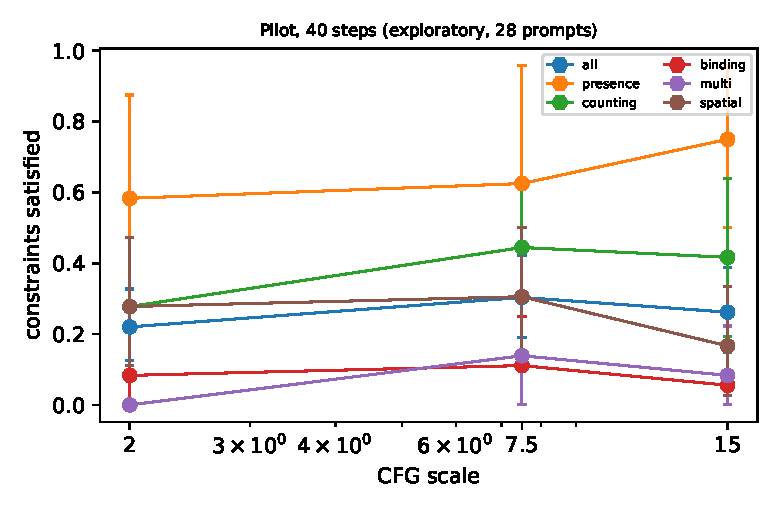
\includegraphics[width=0.7\linewidth]{figures/pilot_adherence.pdf}\caption{Pilot constraint satisfaction against CFG (40 steps, exploratory).}\label{fig:pilot}\end{figure}
\begin{table}[t]
\centering\small
\caption{Pilot (28 prompts, detector-based labels, exploratory): fraction of constraints satisfied, by category, CFG and inference steps; 95\% prompt-cluster bootstrap intervals.}
\label{tab:pilot-adherence}
\begin{tabular}{llrrr}
\toprule
Category & CFG & 20 steps & 40 steps & Prompts \\
\midrule
all & 2 & 0.24 [0.137, 0.351] & 0.22 [0.125, 0.327] & 28 \\
all & 7.5 & 0.30 [0.190, 0.417] & 0.30 [0.190, 0.423] & 28 \\
all & 15 & 0.32 [0.202, 0.440] & 0.26 [0.149, 0.387] & 28 \\
presence & 2 & 0.58 [0.292, 0.875] & 0.58 [0.292, 0.875] & 4 \\
presence & 7.5 & 0.71 [0.417, 0.958] & 0.62 [0.292, 0.958] & 4 \\
presence & 15 & 0.67 [0.292, 1.000] & 0.75 [0.500, 0.958] & 4 \\
counting & 2 & 0.36 [0.167, 0.583] & 0.28 [0.111, 0.472] & 6 \\
counting & 7.5 & 0.39 [0.194, 0.611] & 0.44 [0.250, 0.639] & 6 \\
counting & 15 & 0.44 [0.250, 0.639] & 0.42 [0.194, 0.639] & 6 \\
binding & 2 & 0.06 [0.000, 0.194] & 0.08 [0.000, 0.222] & 6 \\
binding & 7.5 & 0.11 [0.000, 0.278] & 0.11 [0.000, 0.250] & 6 \\
binding & 15 & 0.17 [0.028, 0.333] & 0.06 [0.000, 0.167] & 6 \\
multi & 2 & 0.00 [0.000, 0.000] & 0.00 [0.000, 0.000] & 6 \\
multi & 7.5 & 0.11 [0.000, 0.333] & 0.14 [0.000, 0.306] & 6 \\
multi & 15 & 0.08 [0.000, 0.250] & 0.08 [0.000, 0.223] & 6 \\
spatial & 2 & 0.31 [0.111, 0.500] & 0.28 [0.111, 0.472] & 6 \\
spatial & 7.5 & 0.31 [0.139, 0.500] & 0.31 [0.111, 0.500] & 6 \\
spatial & 15 & 0.33 [0.167, 0.528] & 0.17 [0.028, 0.333] & 6 \\
\bottomrule
\end{tabular}
\par\smallskip\footnotesize Intervals resample prompts; the judge is unaudited on the DEV set.
\end{table}

\begin{table}[t]
\centering\small
\caption{Pilot CFG contrasts (paired by prompt and seed; Holm-adjusted $p$ from Wilcoxon tests), exploratory.}
\label{tab:pilot-cfg}
\begin{tabular}{llrrrr}
\toprule
Category & CFG a vs b & Diff. & 95\% CI & Prompts & $p_{Holm}$ \\
\midrule
presence & 2 vs 7.5 & -0.083 & [-0.438, 0.229] & 4 & 1.000 \\
presence & 2 vs 15 & -0.125 & [-0.500, 0.250] & 4 & 1.000 \\
presence & 7.5 vs 15 & -0.042 & [-0.208, 0.104] & 4 & 1.000 \\
binding & 2 vs 7.5 & -0.042 & [-0.181, 0.097] & 6 & 1.000 \\
binding & 2 vs 15 & -0.042 & [-0.153, 0.083] & 6 & 1.000 \\
binding & 7.5 vs 15 & +0.000 & [-0.111, 0.125] & 6 & 1.000 \\
counting & 2 vs 7.5 & -0.097 & [-0.292, 0.083] & 6 & 1.000 \\
counting & 2 vs 15 & -0.111 & [-0.333, 0.083] & 6 & 1.000 \\
counting & 7.5 vs 15 & -0.014 & [-0.097, 0.056] & 6 & 1.000 \\
spatial & 2 vs 7.5 & -0.014 & [-0.167, 0.153] & 6 & 1.000 \\
spatial & 2 vs 15 & +0.042 & [-0.069, 0.125] & 6 & 0.750 \\
spatial & 7.5 vs 15 & +0.056 & [-0.069, 0.181] & 6 & 1.000 \\
multi & 2 vs 7.5 & -0.125 & [-0.292, 0.000] & 6 & 0.750 \\
multi & 2 vs 15 & -0.083 & [-0.222, 0.000] & 6 & 1.000 \\
multi & 7.5 vs 15 & +0.042 & [-0.083, 0.208] & 6 & 1.000 \\
all & 2 vs 7.5 & -0.071 & [-0.155, 0.009] & 28 & 0.174 \\
all & 2 vs 15 & -0.060 & [-0.146, 0.018] & 28 & 0.214 \\
all & 7.5 vs 15 & +0.012 & [-0.045, 0.071] & 28 & 0.873 \\
\bottomrule
\end{tabular}
\end{table}

Global attention re-weighting (scale~2 against the control path) changed overall adherence by \intAllDiff{} (95\% CI \intAllLo{} to \intAllHi{}), i.e.\ no resolved improvement (Table~\ref{tab:pilot-intervention}).
\begin{table}[t]
\centering\small
\caption{Pilot global attention re-weighting (scale 2 and 4 against the scale-1 control path), primary outcome, exploratory.}
\label{tab:pilot-intervention}
\begin{tabular}{llrrrr}
\toprule
Category & Arm & Diff. & 95\% CI & Prompts & $p_{Holm}$ \\
\midrule
presence & rw2 vs control & +0.167 & [0.000, 0.375] & 4 & 0.500 \\
presence & rw4 vs control & +0.125 & [-0.042, 0.333] & 4 & 0.500 \\
binding & rw2 vs control & +0.028 & [-0.111, 0.167] & 6 & 1.000 \\
binding & rw4 vs control & +0.028 & [-0.139, 0.222] & 6 & 1.000 \\
counting & rw2 vs control & +0.028 & [0.000, 0.111] & 6 & 1.000 \\
counting & rw4 vs control & +0.028 & [-0.083, 0.139] & 6 & 1.000 \\
spatial & rw2 vs control & -0.028 & [-0.194, 0.139] & 6 & 1.000 \\
spatial & rw4 vs control & +0.056 & [-0.139, 0.250] & 6 & 1.000 \\
multi & rw2 vs control & -0.028 & [-0.194, 0.111] & 6 & 1.000 \\
multi & rw4 vs control & -0.083 & [-0.222, 0.000] & 6 & 1.000 \\
all & rw2 vs control & +0.024 & [-0.042, 0.089] & 28 & 0.757 \\
all & rw4 vs control & +0.024 & [-0.054, 0.095] & 28 & 0.757 \\
\bottomrule
\end{tabular}
\par\smallskip\footnotesize Control images were pixel-identical to the unmodified pipeline (owner-documented 168/168).
\end{table}

Among binding-bearing pilot images, all required objects were detected in \pilotEligibleN{} of \pilotBindingN{} (\pilotEligible{}), but only \pilotEligibleBMN{} of \pilotBindingBMN{} (\pilotEligibleBM{}) for the binding and multi categories, because counting prompts are always eligible; the pilot's legacy binding score already counts omissions as failures. In prompt-grouped cross-validation, early attention features added $\Delta$AUC of \dAucAttnNoise{} (95\% CI \dAucAttnNoiseLo{} to \dAucAttnNoiseHi{}) over the design and seed baseline, whereas seed identity added \dAucNoiseDesign{} (Table~\ref{tab:pilot-nested}); only six distinct noise vectors exist in the pilot, a seed-0 deficit appeared (permutation $p=\seedP$), and both are post hoc observations. They motivated an earlier protocol revision's question of whether attention is a forecast or a read-out of the outcome (then labelled HB). The current revision demoted that question to a supporting analysis outside the registered family (HA, HD, HE, HF); Section~\ref{sec:resATTN} revisits it descriptively.
\begin{table}[t]
\centering\small
\caption{Pilot nested prediction of the primary outcome (40-step images, prompt-grouped cross-validation, 28 prompts); exploratory.}
\label{tab:pilot-nested}
\begin{tabular}{lrr}
\toprule
Contrast & $\Delta$AUC & 95\% prompt-bootstrap CI \\
\midrule
attn\_minus\_design & +0.067 & [0.028, 0.122] \\
noise\_minus\_design & +0.002 & [-0.028, 0.027] \\
attn\_minus\_noise & +0.050 & [0.017, 0.097] \\
\bottomrule
\end{tabular}
\par\smallskip\footnotesize Base rate 0.236. Only six distinct noise vectors exist in the pilot, so noise features equal seed identity (noise vs design: -0.007).
\end{table}


\subsection{B. Infrastructure and integrity (not scientific findings)}
On a Tesla T4 with the committed code, the GPU identity script ran \rZeroCases{} cases and \rZeroHold{} (determinism, loop from step 0, reload-and-resume, zero-magnitude branch, hook-off control, restored baseline; maximum pixel difference $0$). The scope is three pilot prompts at one seed and setting; the model revision is not recorded inside that artifact. The R2a DEV core contains $400$ images and \rTwoLatents{} saved checkpoints; an independent audit passed \rTwoPassed{} of \rTwoChecks{} hard checks (manifest coverage, hashes, readability, no duplicates or orphans, checkpoint layout). A one-sample-pair regeneration on a different GPU matched the stored latent at the same step best, supporting the checkpoint indexing; this was not a bit-level Kaggle comparison. Two throughput probes disagree by about $25\%$ (Table~\ref{tab:throughput}) and are not reconciled.
\begin{table}[t]
\centering\small
\caption{Measured throughput on Tesla T4 (seconds per 40-step image, first image excluded) from two probe sessions; the real R2a run gave a median of 6.21 and 6.26 s per worker.}
\label{tab:throughput}
\begin{tabular}{lrrr}
\toprule
Session & Plain & With latents & Two workers, wall (s) \\
\midrule
R1 session 10:10 UTC & 6.16 & 6.25 & 53.9 \\
R0 session 15:02 UTC & 7.76 & 7.59 & 60.5 \\
\bottomrule
\end{tabular}
\end{table}


\subsection{C. First-pass DEV outcomes (unaudited judge)}
\begin{table}[t]
\centering\small
\caption{R2a DEV core, first-pass detector (J1) outcomes on binding-bearing canonical prompts. \textbf{Unaudited judge; exploratory.}}
\label{tab:r2a-first-pass}
\begin{tabular}{lrr}
\toprule
Quantity & Value & n \\
\midrule
All required objects detected & 0.404 & 280 \\
Binding given presence & 0.487 & 113 \\
Joint (present and bound) & 0.196 & 280 \\
\bottomrule
\end{tabular}
\par\smallskip\footnotesize 70 scenes $\times$ 4 seeds. These outcomes precede the judge audit (\S\ref{sec:evaluation}).
\end{table}

Only about \rTwoPres{} of binding-bearing DEV images have every required object detected and binding given presence is defined for \rTwoEligN{} of \rTwoBB{} images. Whether this reflects the model or the detector cannot be said before the audit.
